\documentclass[12pt]{article}

\usepackage{paper,math}
\usepackage[margin=1in]{geometry}
\addbibresource{references.bib}
\usepackage{xcolor}  % To define colors like mygr
\usepackage[most]{tcolorbox}  % For colored boxes
\usepackage{tikz} 
\usepackage{algorithm}% http://ctan.org/pkg/algorithms
\usepackage{algpseudocode}% http://ctan.org/pkg/algorithmicx
\usepackage{algorithmicx}
\renewcommand{\figurename}{Abbildung} % Repeat for appendix if required
\renewcommand{\tablename}{Tabelle} % Repeat for appendix if required


\newcommand{\malte}[1]{\coauthorComment[Malte]{#1}}

\definecolor{gre}{RGB}{101, 191, 127}
\definecolor{gree}{RGB}{7, 135, 44}

\newtcolorbox{defin}[2][]{colback=mygr!10,enhanced,title= #2,#1,
attach boxed title to top left={xshift=-4mm},boxrule=0pt,after skip=1cm,before skip=1cm,right skip=0cm,breakable,fonttitle=\bfseries,toprule=0pt,bottomrule=0pt,rightrule=0pt,leftrule=4pt,arc=0mm,skin=enhancedlast jigsaw,sharp corners,colframe=mygr,colbacktitle=mygr,boxed title style={
	frame code={ 
		\fill[mygr](frame.south west)--(frame.north west)--(frame.north east)--([xshift=3mm]frame.east)--(frame.south east)--cycle;
		\draw[line width=1mm,mygr]([xshift=2mm]frame.north east)--([xshift=5mm]frame.east)--([xshift=2mm]frame.south east);
		
		\draw[line width=1mm,mygr]([xshift=5mm]frame.north east)--([xshift=8mm]frame.east)--([xshift=5mm]frame.south east);
		\fill[mygr!40](frame.south west)--+(4mm,-2mm)--+(4mm,2mm)--cycle;
	}
}
}

\definecolor{mygr}{HTML}{2C3338}



\title{Genomorientierte Bioinformatik \\ - \\ BamFeatures}
\author{Malte Weyrich}
\date{\today}
% Conditionally display thoughts (hide by switching to `\boolfalse`)
% \booltrue{INCLUDECOMMENTS}
\begin{document}

% Title Page -------------------------------------------------------------------
\maketitle
\begin{abstract}
Das Sequenzieren in der Bioinformatik generiert Milliarden von \textit{Reads} pro \textit{Sample}, welche mit
einem \textit{Mapper} an das \textit{Referenzgenom} aligniert werden. 
Diese Daten werden in einer \textit{Sequence Alignment Map (SAM)} gespeichert und können zusätzlich in ein komprimiertes Format,
einer \textit{Binary Alignment Map (BAM)} Datei, umgewandelt werden. Anschließend können verschiedene Analysen auf
den \textit{BAM} Dateien durchgeführt werden. Die in diesem Report diskutierte \textit{JAR} liest eine gegebene
\textit{paired-end RNA-seq BAM} Datei ein und errechnet verschiedene Features, die in einer \textit{<tsv>} Datei
gespeichert werden. Die JAR wurde auf drei verschiedenen \textit{BAM} Dateien ausgeführt, um damit
anschießend die \textit{RPKM} Werte zu berechnen. Zudem wird die \textit{JAR} anhand ihrer Laufzeit und
Korrektheit analysiert.

\end{abstract}

\newpage


% Paper ------------------------------------------------------------------------

% ------------------------------------------------------------------------------
% ------------------------------------------------------------------------------
\section{RNA-seq}
Die Bezeichnung \textit{RNA-seq} bezieht sich auf ein bestimmtes Sequenzierprotokoll der Bioinformatik bei dem
möglichst alle exprimierten Transkripte mehrerer Samples mittels Hochdurchsatz-sequenziergeräten wie
\textit{Illumina} verarbeitet und die resultierenden \textit{Reads} in Ausgabe Dateien abgespeichert werden.
Bei \textit{Illumina} werden die extrahierten Transkripte mittels Ultraschall oder enzymatischer Fermentation in Fragmente mit ähnlicher Länge
zerstückelt und mit Adaptersequenzen und Barcodes versehen. Darauf folgt eine \textit{PCR} Amplifikation der 
Fragmente, um das Signal zu verstärken. Die amplifizierten Fragmente können nun im Sequenzierzyklus 
von \textit{Illumina}, Base für Base, gelesen werden. Dabei wird jedoch nicht das ganze Fragment gelesen, sondern
jeweils nur ca. $100BP$ (abhängig von Voreinstellung und Protokoll) beider Enden des Fragments (\textit{paired-end sequencing}).
Somit entstehen pro Fragment zwei \textit{Reads}, ein forward \textit{Read} und ein reverse \textit{Read},
welche zu einem \textit{ReadPair} zusammengefasst werden können. 
In dem Protokoll von \textit{Illumina} werden zuerst alle \textit{Reads} eines Endes aller
Fragmente gemacht, dann wird das Fragment, \textbf{vereinfacht gesagt}, auf der \textit{Flow Zelle} umgedreht (durch Replikation), wodurch 
die umgedrehten Fragmente jeweils das Komplement ihres ursprünglichen Fragments sind.
Somit sollten die \textit{Reads} eines \textit{ReadPairs} immer auf entgegengesetzte Stränge \textit{("+"/"-")}
\textit{"mappen"}. Ist bei einem Sequenzierexperiment die Ausgangskonfiguration der Fragmente bekannt, so handelt 
es sich um ein \textit{strand specific} Experiment und man kann allen
\textit{Reads} einem festen Strang zuordnen, je nach dem, ob das Fragment in der Anfangskonfiguration
vom \textit{"-"} oder vom \textit{"+"} Strang kam.
Ein \textit{Mapper} würde nun solche \textit{ReadPairs} an einem \textit{Referenzgenom} \textit{mappen}
und eine (oder mehrere) \textit{SAM/BAM} Datei(en) erstellen, welche unter anderem die Koordinaten der alignierten 
\textit{Reads} basierend auf dem \textit{Referenzgenom} beinhalten. 
Die Alignment Daten dieser Datei können nun von der \textit{BamFeatures JAR} weiter annotiert werden. 


\section{Java Programm}
\begin{verbatim*}
Usage:
    java -jar bam.jar -bam <bamPath> -o <outputPath> -gtf <gtfPath> \\
                      [-frstrand <true/false>] [-lengths]
\end{verbatim*}
\subsection{Argumente}
Zusätzlich zu den vorausgesetzten Argumenten (\textit{-bam}, \textit{-o}, \textit{-gtf}) können noch \textit{-frstrand} und
\textit{-lengths} angegeben werden. 
Bei einem Strangpositiven Experiment (\textit{-frstrand true}) ist der forward \textit{Read} auf dem \textit{"+"} und der reverse \textit{Read} auf dem
\textit{"-"}. So kann die \textit{JAR} die \textit{Reads} korrekt zuordnen. 
Falls die Strangrichtung nicht angegeben ist, werden für beide \textit{Reads} jeweils beide Stränge betrachtet.
Die \textit{-lengths} Option wird für die Berechnung der \textit{RPKM} Werte benötigt. 
Ist diese Option gesetzt, so werden die für die Längennormalisierung benötigte Genlängen der kombinierten Exons jedes
Gens berechnet und in einer \textit{<tsv>} Datei gespeichert.
\subsection{Logik}
\subsubsection{Erstellen der ReadPair Objekte}

Die Einträge der \textit{BAM} Datei werden der Reihe nach von einem \textit{SAMFilereader} eingelesen. Da es
sich um \textit{paired-end} Daten handelt, muss für jeden \textit{Read} sein zugehöriger \textit{Mate} gefunden werden. 
Reads die nicht gepaart sind, oder nicht den Qualitätsanforderungen der Aufgabenstellung entsprechen,
werden ignoriert.
\textit{Read Objekte} die zum ersten Mal vorkommen, werden in einer \\ \textit{HashMap<Id, Read> seenEntries}
gespeichert und für jede Iteration wird überprüft, ob wir die \textit{Read Id} bereits gesehen haben.
Sobald wir zwei zusammengehörende \textit{Reads} identifiziert haben, wird ein neues
\textit{ReadPair Objekt} erstellt. Dabei wird die Strangrichtung beim erstellen des Objekts berücksichtigt und
die \textit{Reads} jeweils nach \textit{forward} und \textit{reverse} kategorisiert.
\newpage

\subsubsection{Berechnung der ReadPair Attribute}
Als erstes werden die \textit{igenes} und \textit{cgenes} berechnet:
\begin{enumerate}
    \item \textit{cgenes} := $\left\{g \in \textit{cgenes} \hspace{1mm}|\hspace{1mm} g_{start } < fwRead_{start} \land g_{end} > rwRead_{end}\right\}$
    \item \textit{igenes} := $\left\{g \in \textit{igenes} \hspace{1mm}|\hspace{1mm} g_{start} >= fwRead_{start} \land g_{end} <= rwRead_{end}\right\}$
\end{enumerate}
Für die Berechnung dieser Attribute verwenden wir ein verschachteltes Objekt \textit{intervalTreeMap} \textit{HashMap<String, HashMap<Boolean, IntervalTree<Gene>\hspace{0.1mm}>\hspace{0.1mm}>}
verwendet, welches für jedes Chromosom die Gene nach ihrem Strang in Intervalbäumen abgespeichert hat (Strang ist entweder: [\textit{true}|\textit{false}|\textit{null}]).
Falls \textit{|cgenes|} $== 0$ aber \textit{|igenes|} $> 0$  wird das \textit{ReadPair} verworfen und 
mit dem nächsten weiter gemacht, sind beide Mengen leer, so wird die kürzeste Distanz zu benachbarten Genen ausgerechnet und in
\textit{gdist} abgespeichert.
Danach wird das \textit{ReadPair} auf \textit{split-inconsistency} überprüft, d.h. falls es eine überlappende 
Region beider \textit{Reads} gibt, müssen die potentiell implizierten Introns beider \textit{Reads} übereinstimmen.
\begin{algorithm}[!htbp]
\caption{getNsplit()}
\begin{algorithmic}[1]
\State \textbf{Input:} fw, rw \Comment{forward and reverse reads}
\If{$|\text{fw.Blocks}| = 1$ \textbf{and} $|\text{rw.Blocks}| = 1$}\Comment{Checks if the reads imply introns}
    \State \Return 0 
\EndIf
\State overlap = determineOverlap(fw, rw) \Comment{Determine overlap region}
\State iFwRegions $\gets \{\}$ \Comment{Set for containing fw Introns}
\State iRwRegions $\gets \{\}$ \Comment{Set for containing rw Introns}
\State iRegions $\gets \{\}$ \Comment{Set for containing all Introns}
\State \textbf{extractIntronsInOverlap}(overlap.x1, overlap.x2, iFwRegions, iRegions, fw) 
\State \textbf{extractIntronsInOverlap}(overlap.x1, overlap.x2, iRwRegions, iRegions, rw)
\If{|iRwRegions| $\neq$ |iFwRegions|}
\State \Return -1 \Comment{split-inconsistent}
\EndIf
\If{iRwRegions = iFwRegions}
\State \Return |iRegions|\Comment{Return unique Introns in overlap}
\EndIf
\State \Return -1\Comment{split-inconsistent (default)}
\end{algorithmic}
\end{algorithm}
Nach dem Aufruf von \textit{getNsplit()} wird bei einem \textit{return value} von -1 das \textit{ReadPair} als 
\textit{"split-inconsistent"} vermerkt und in die Ausgabedatei übernommen, ansonsten wird die Grö\ss e der
Menge \textit{iRegions} in der Variable \textit{nsplit} gespeichert und das \textit{ReadPair} weiter prozessiert.
\newpage
Als nächstes wird das \textit{ReadPair} anhand drei Kategorien annotiert \ref{fig:-figures-ReadAnnotation-png}:
\begin{figure}[htpb]
    \centering
    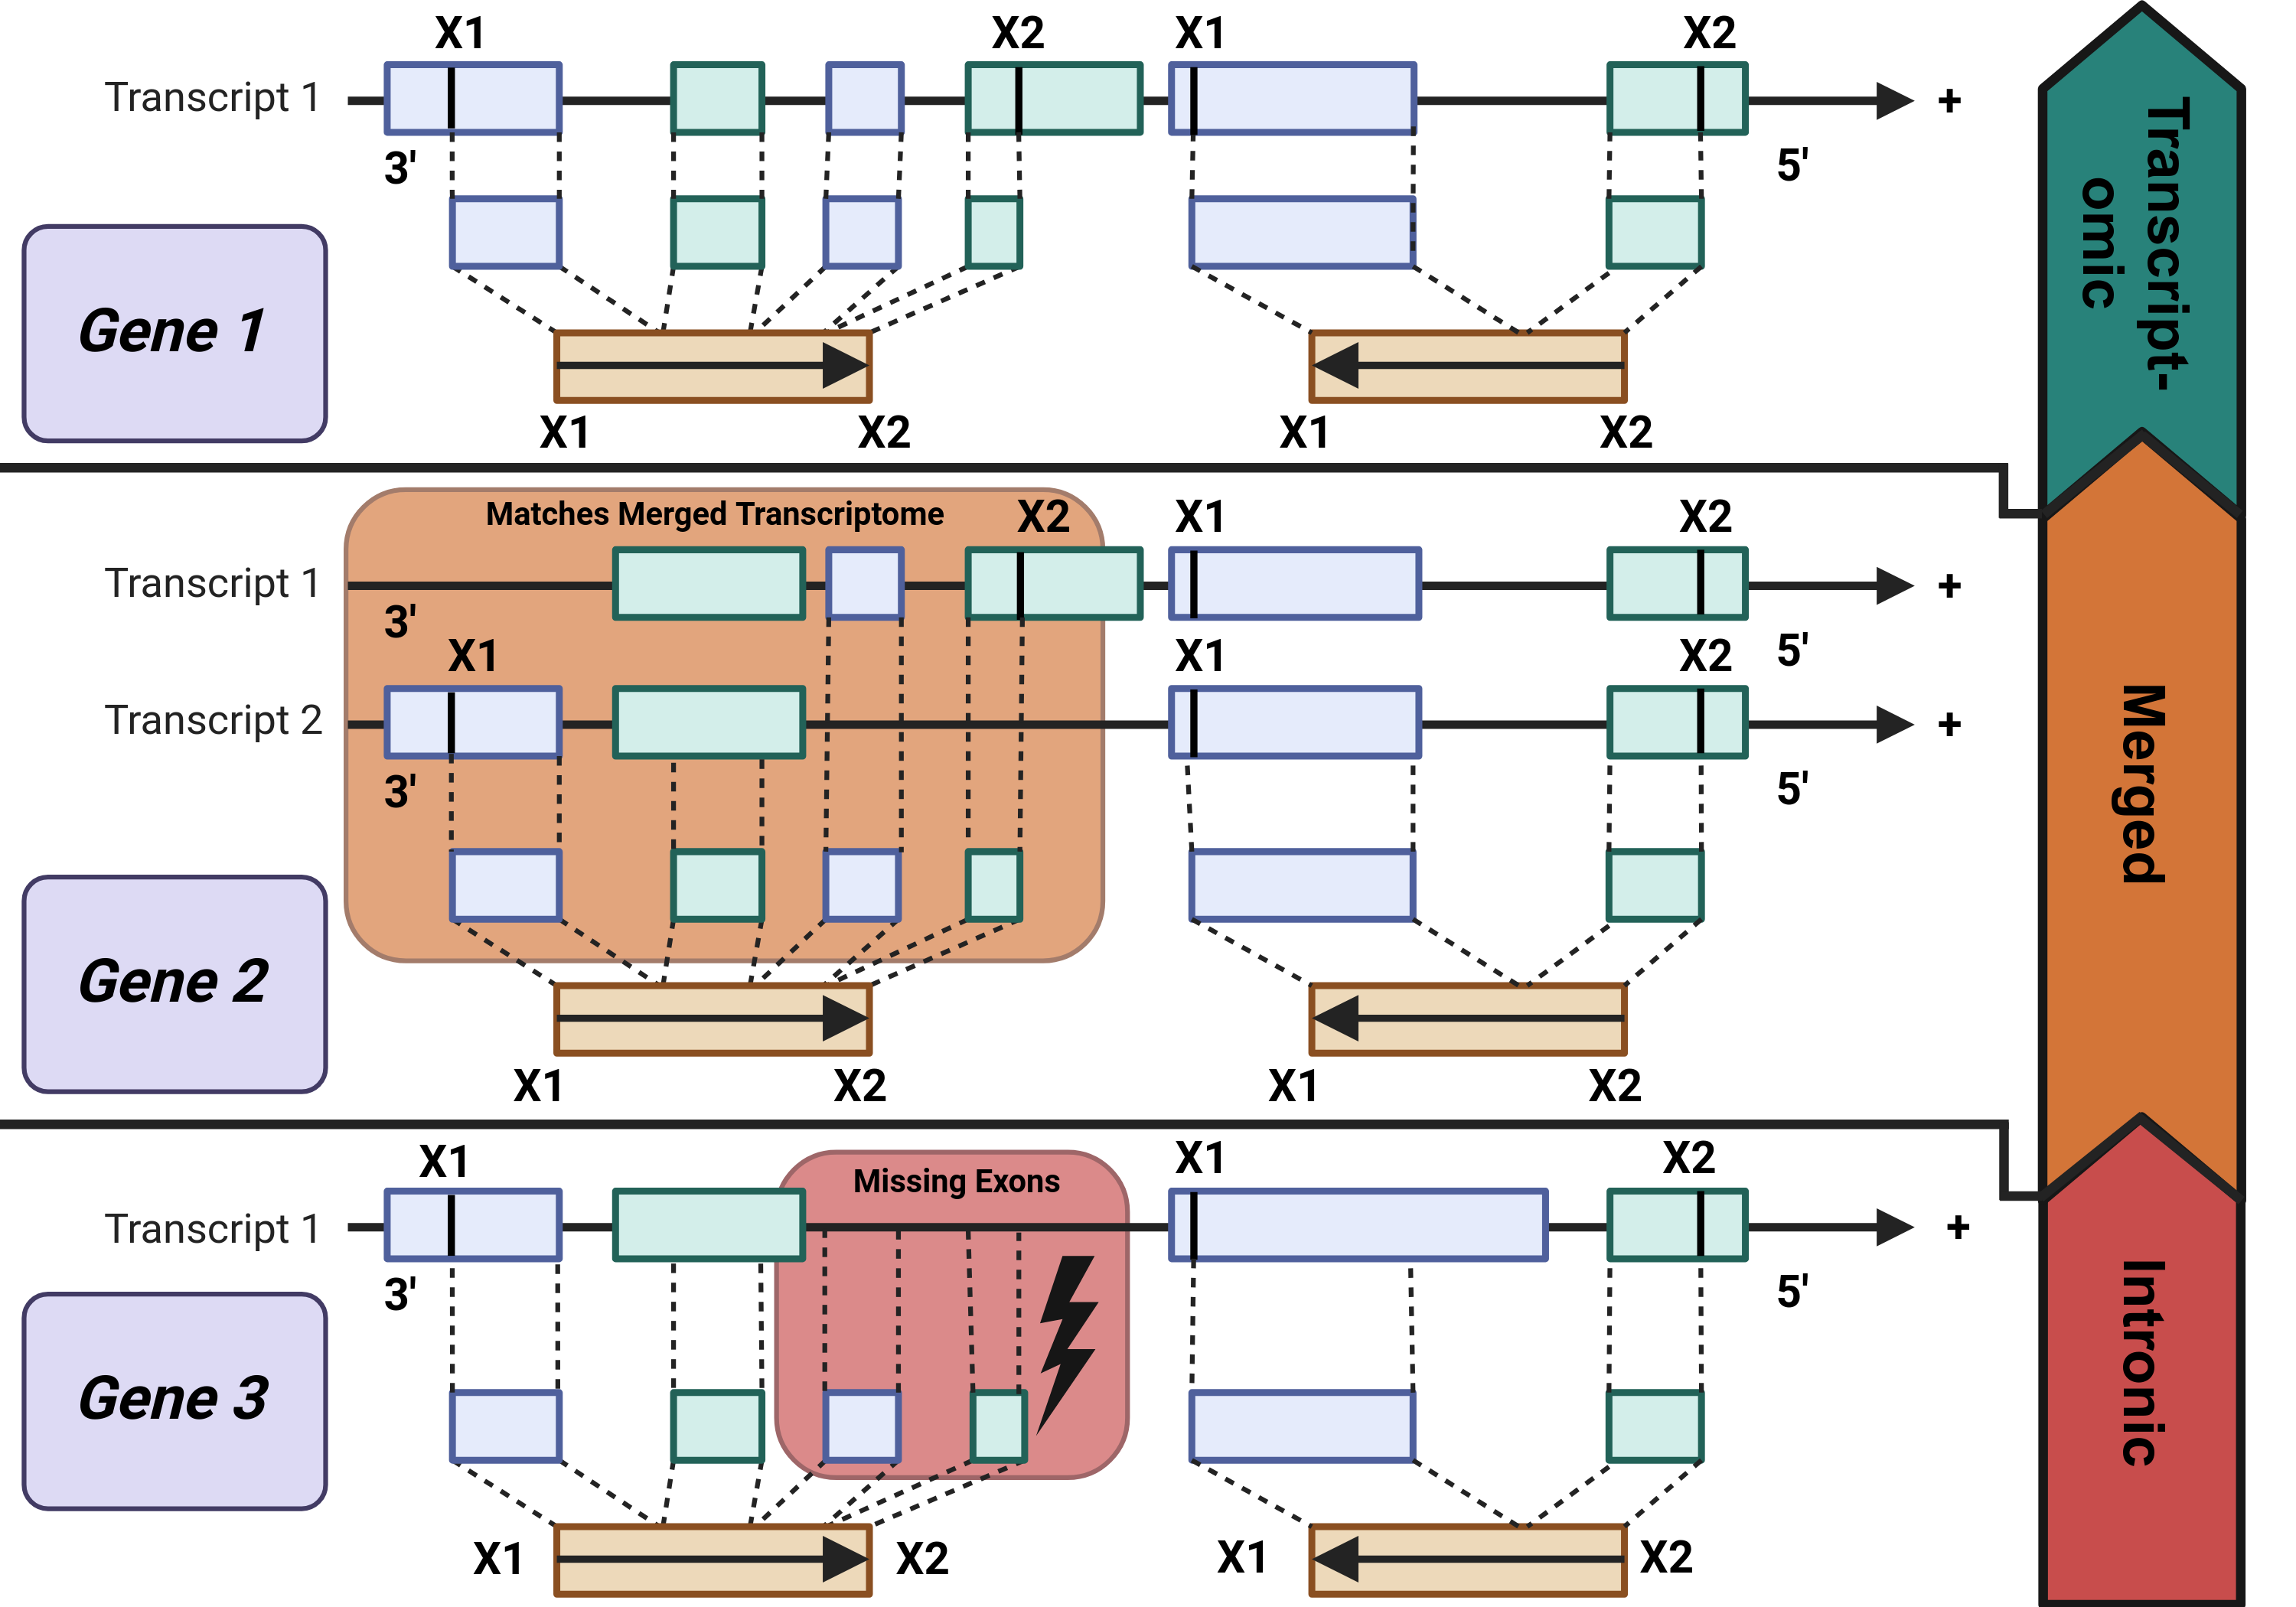
\includegraphics[width=0.95\textwidth]{./figures/ReadAnnotation.png}
\caption{Kategorisierung der \textit{ReadPair}-Regionen in die Klassen \textit{\textbf{"Transcriptomic"}},
\textit{\textbf{"Merged"}} und \textit{\textbf{"Intronic"}}, wobei eine Priorisierung nach 
der Reihenfolge \textit{\textbf{"Transcriptomic"}} > \textit{\textbf{"Merged"}} > \textit{\textbf{"Intronic"}} erfolgt.
Die \textit{AlignmentBlocks} der \textit{Reads} werden mit den Exons der Transkripte des inkludierenden Gens abgeglichen. 
Die Abbildung wurde mit \cite{biorender} erstellt}
    \label{fig:-figures-ReadAnnotation-png}
\end{figure}




\subsection{Laufzeit}
\begin{figure}[htpb]
    \centering
    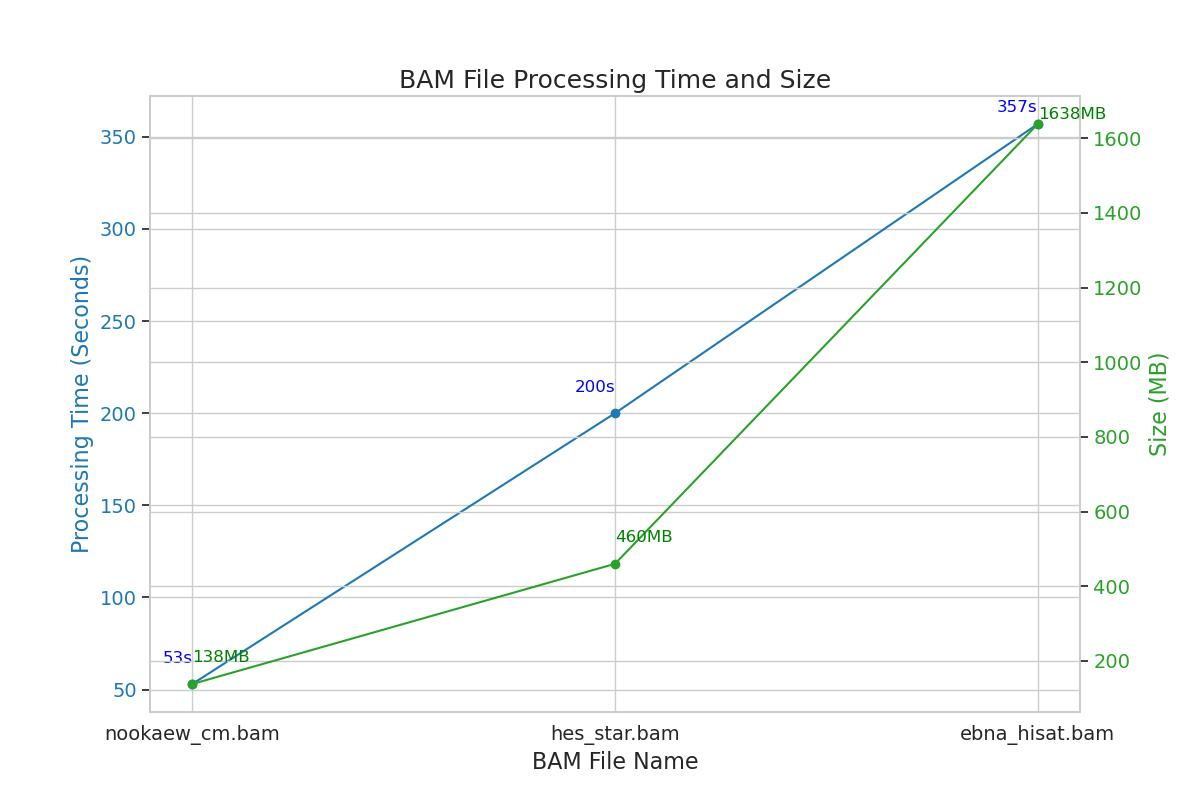
\includegraphics[width=0.9\textwidth]{./plots/times_bam.jpg}
    \caption{Laufzeit der JAR auf den 3 vorgegebenen \textit{BAMs} in Sekunden verglichen mit dem \textit{BAM} Volumen in \textit{MB} }
    \label{fig:-plots-times_bam-jpg}
\end{figure}
\subsection{Korrektheit}
\subsection{Benchmarking}
\section{Ergebnisse}

% \begin{figure}[htpb]
%     \centering
%     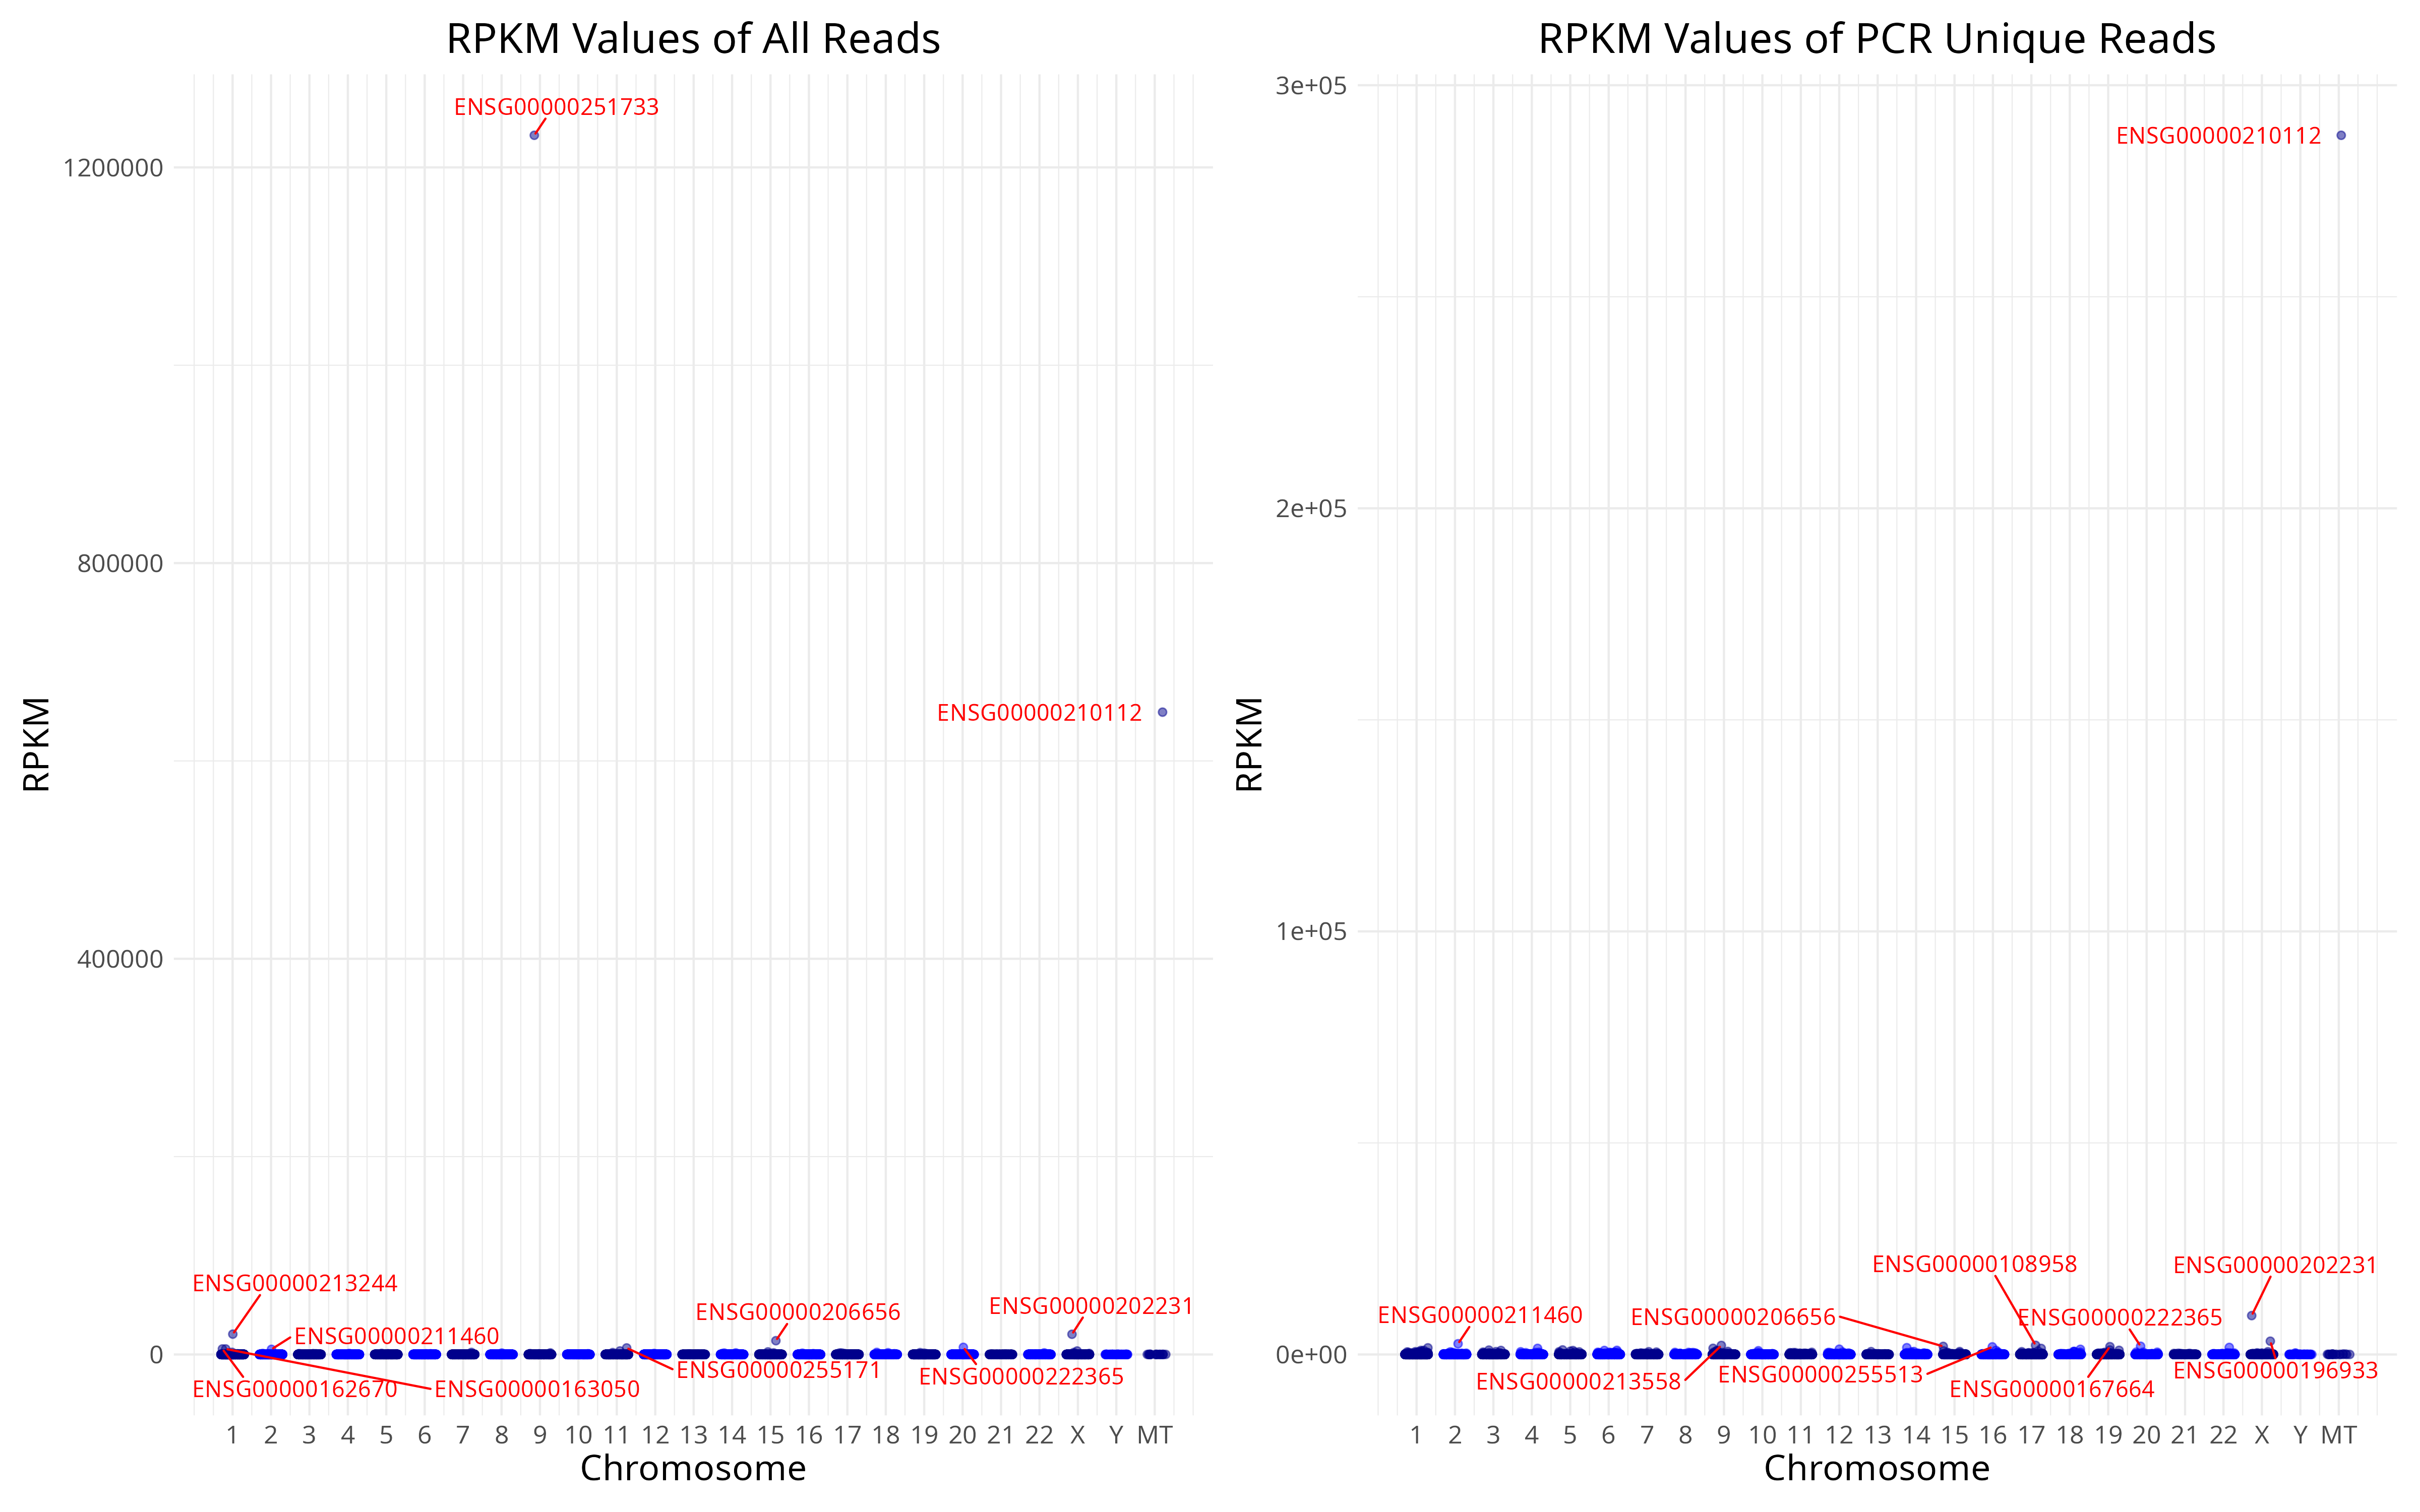
\includegraphics[width=0.85\textwidth]{./plots/hes_star/Plots/rpkm_mplot.png}
%     \caption{}
%     \label{fig:-plots-hes_star-Plots-rpkm_mplot-png}
% \end{figure}
% \begin{figure}[htpb]
%     \centering
%     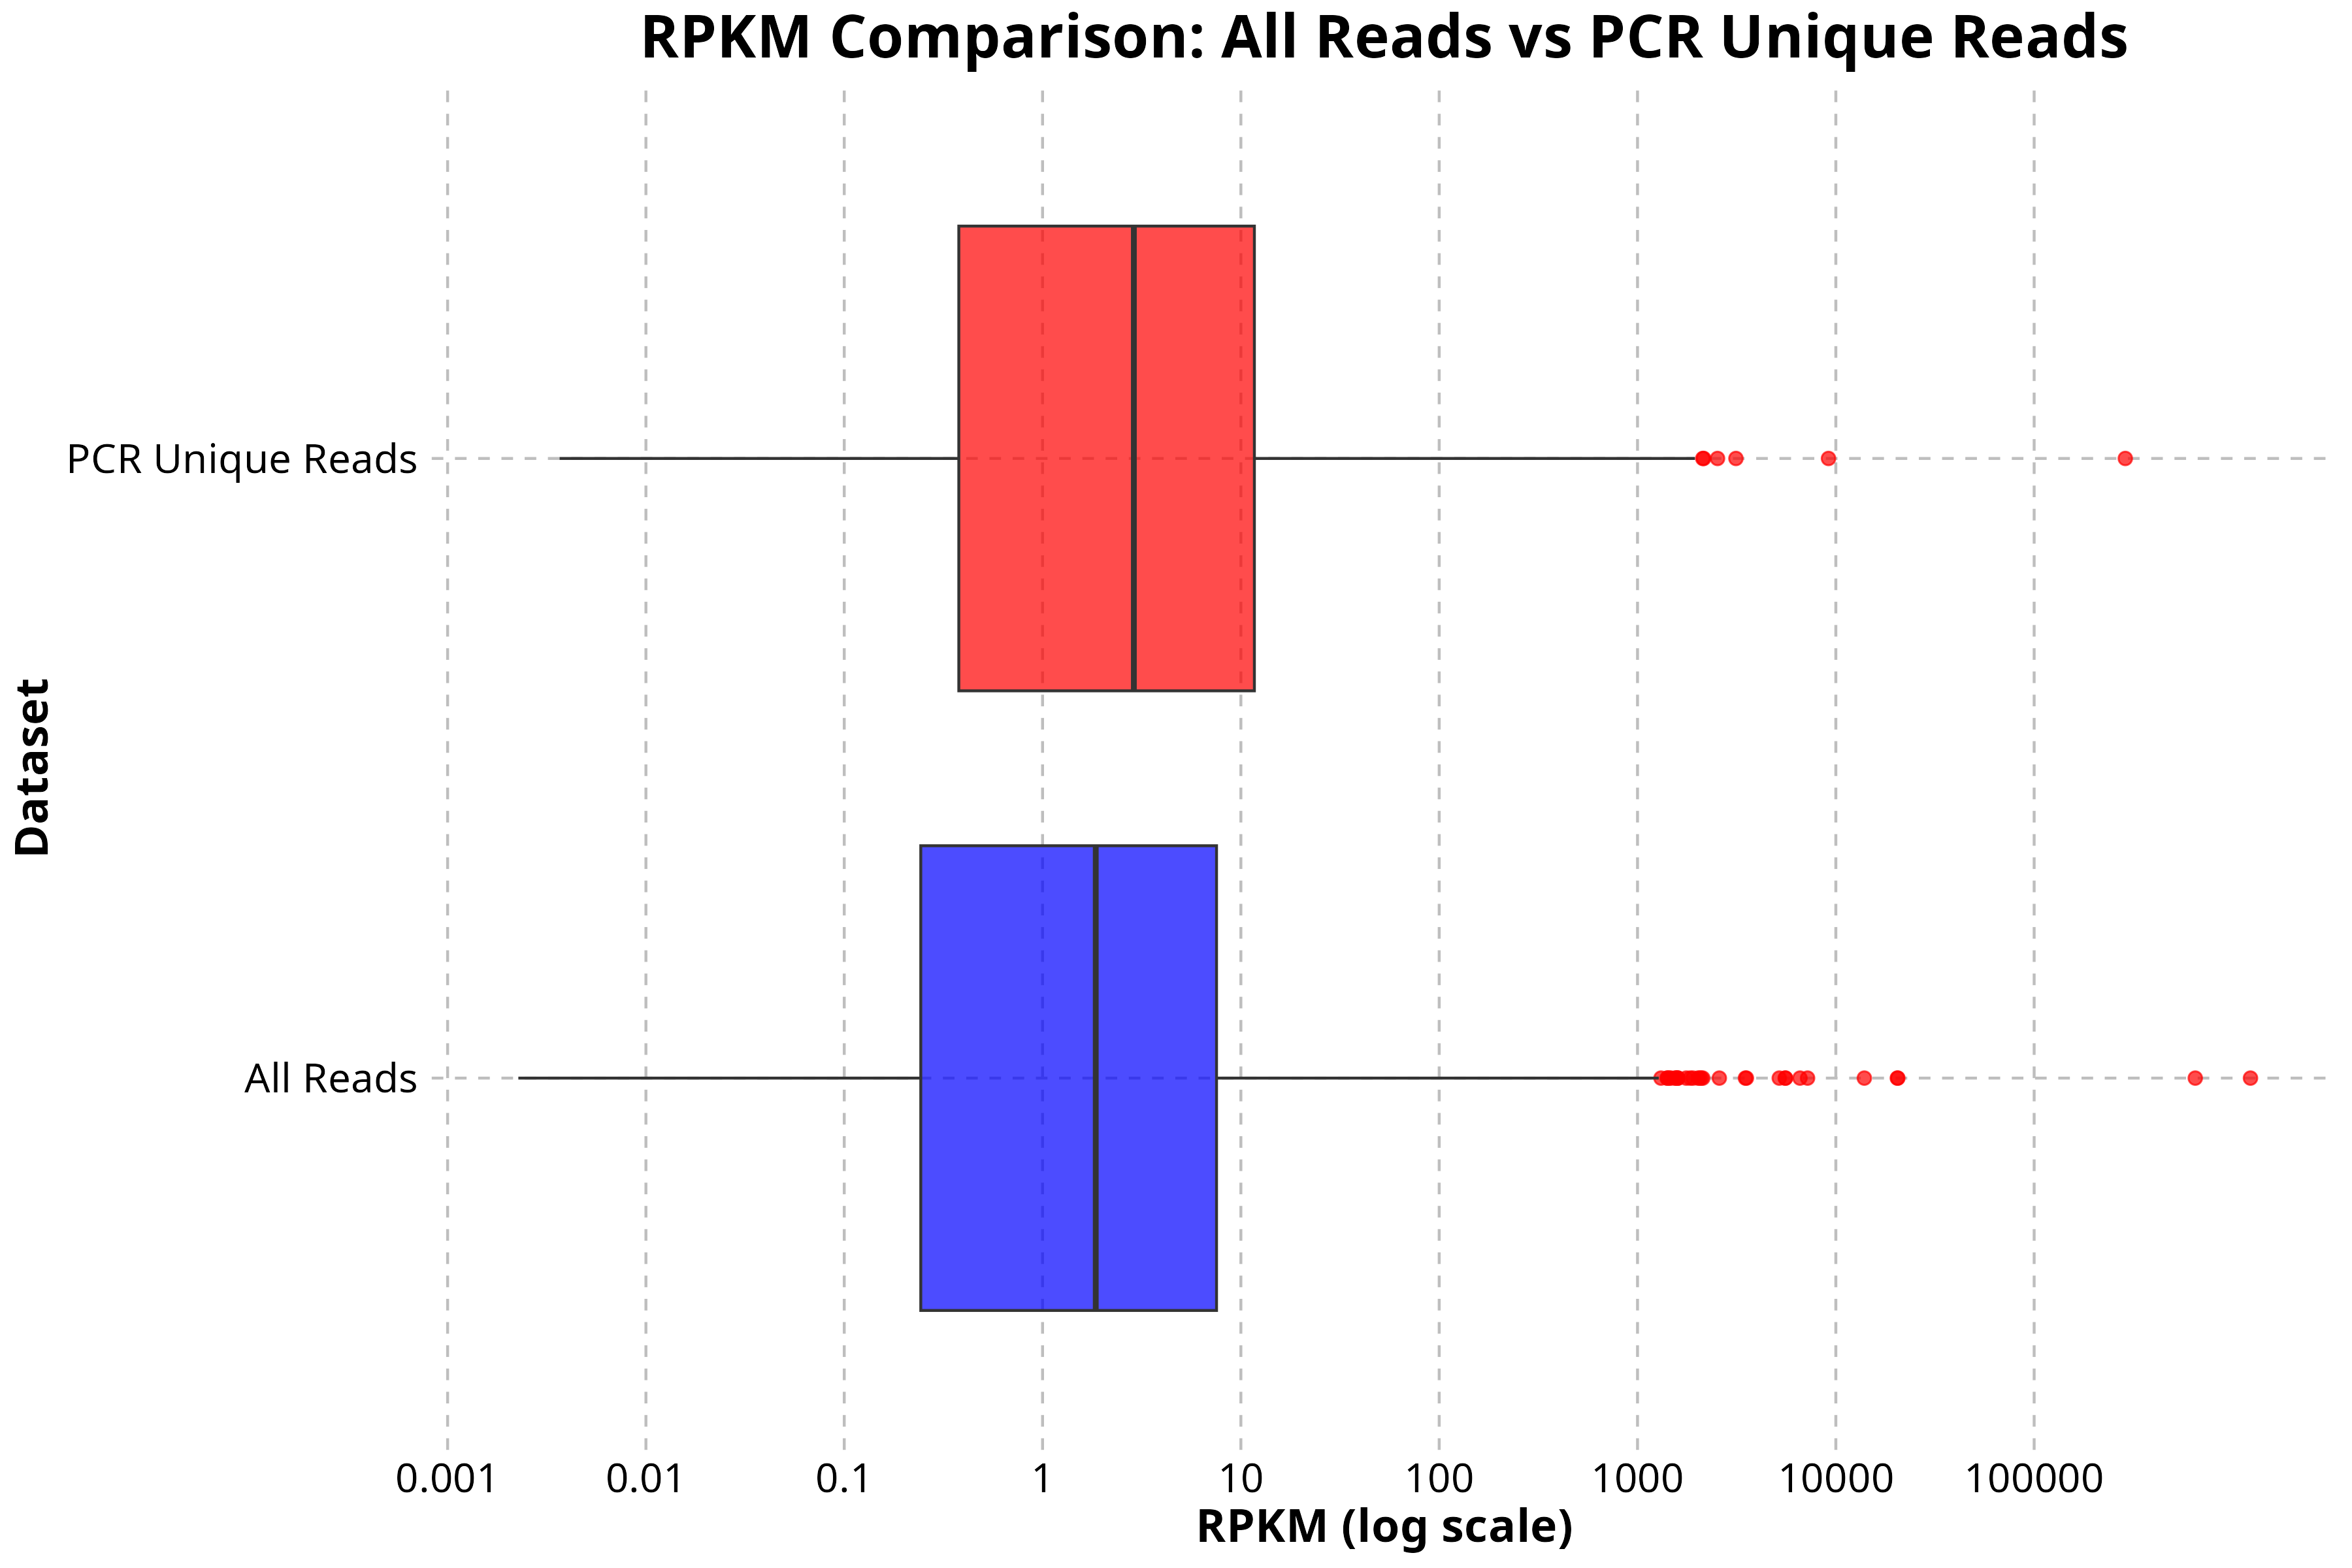
\includegraphics[width=0.85\textwidth]{./plots/hes_star/Plots/rpkm_hist.png}
%     \caption{}
%     \label{fig:-plots-hes_star-Plots-rpkm_hplot-png}
% \end{figure}
% \begin{figure}[htpb]
%     \centering
%     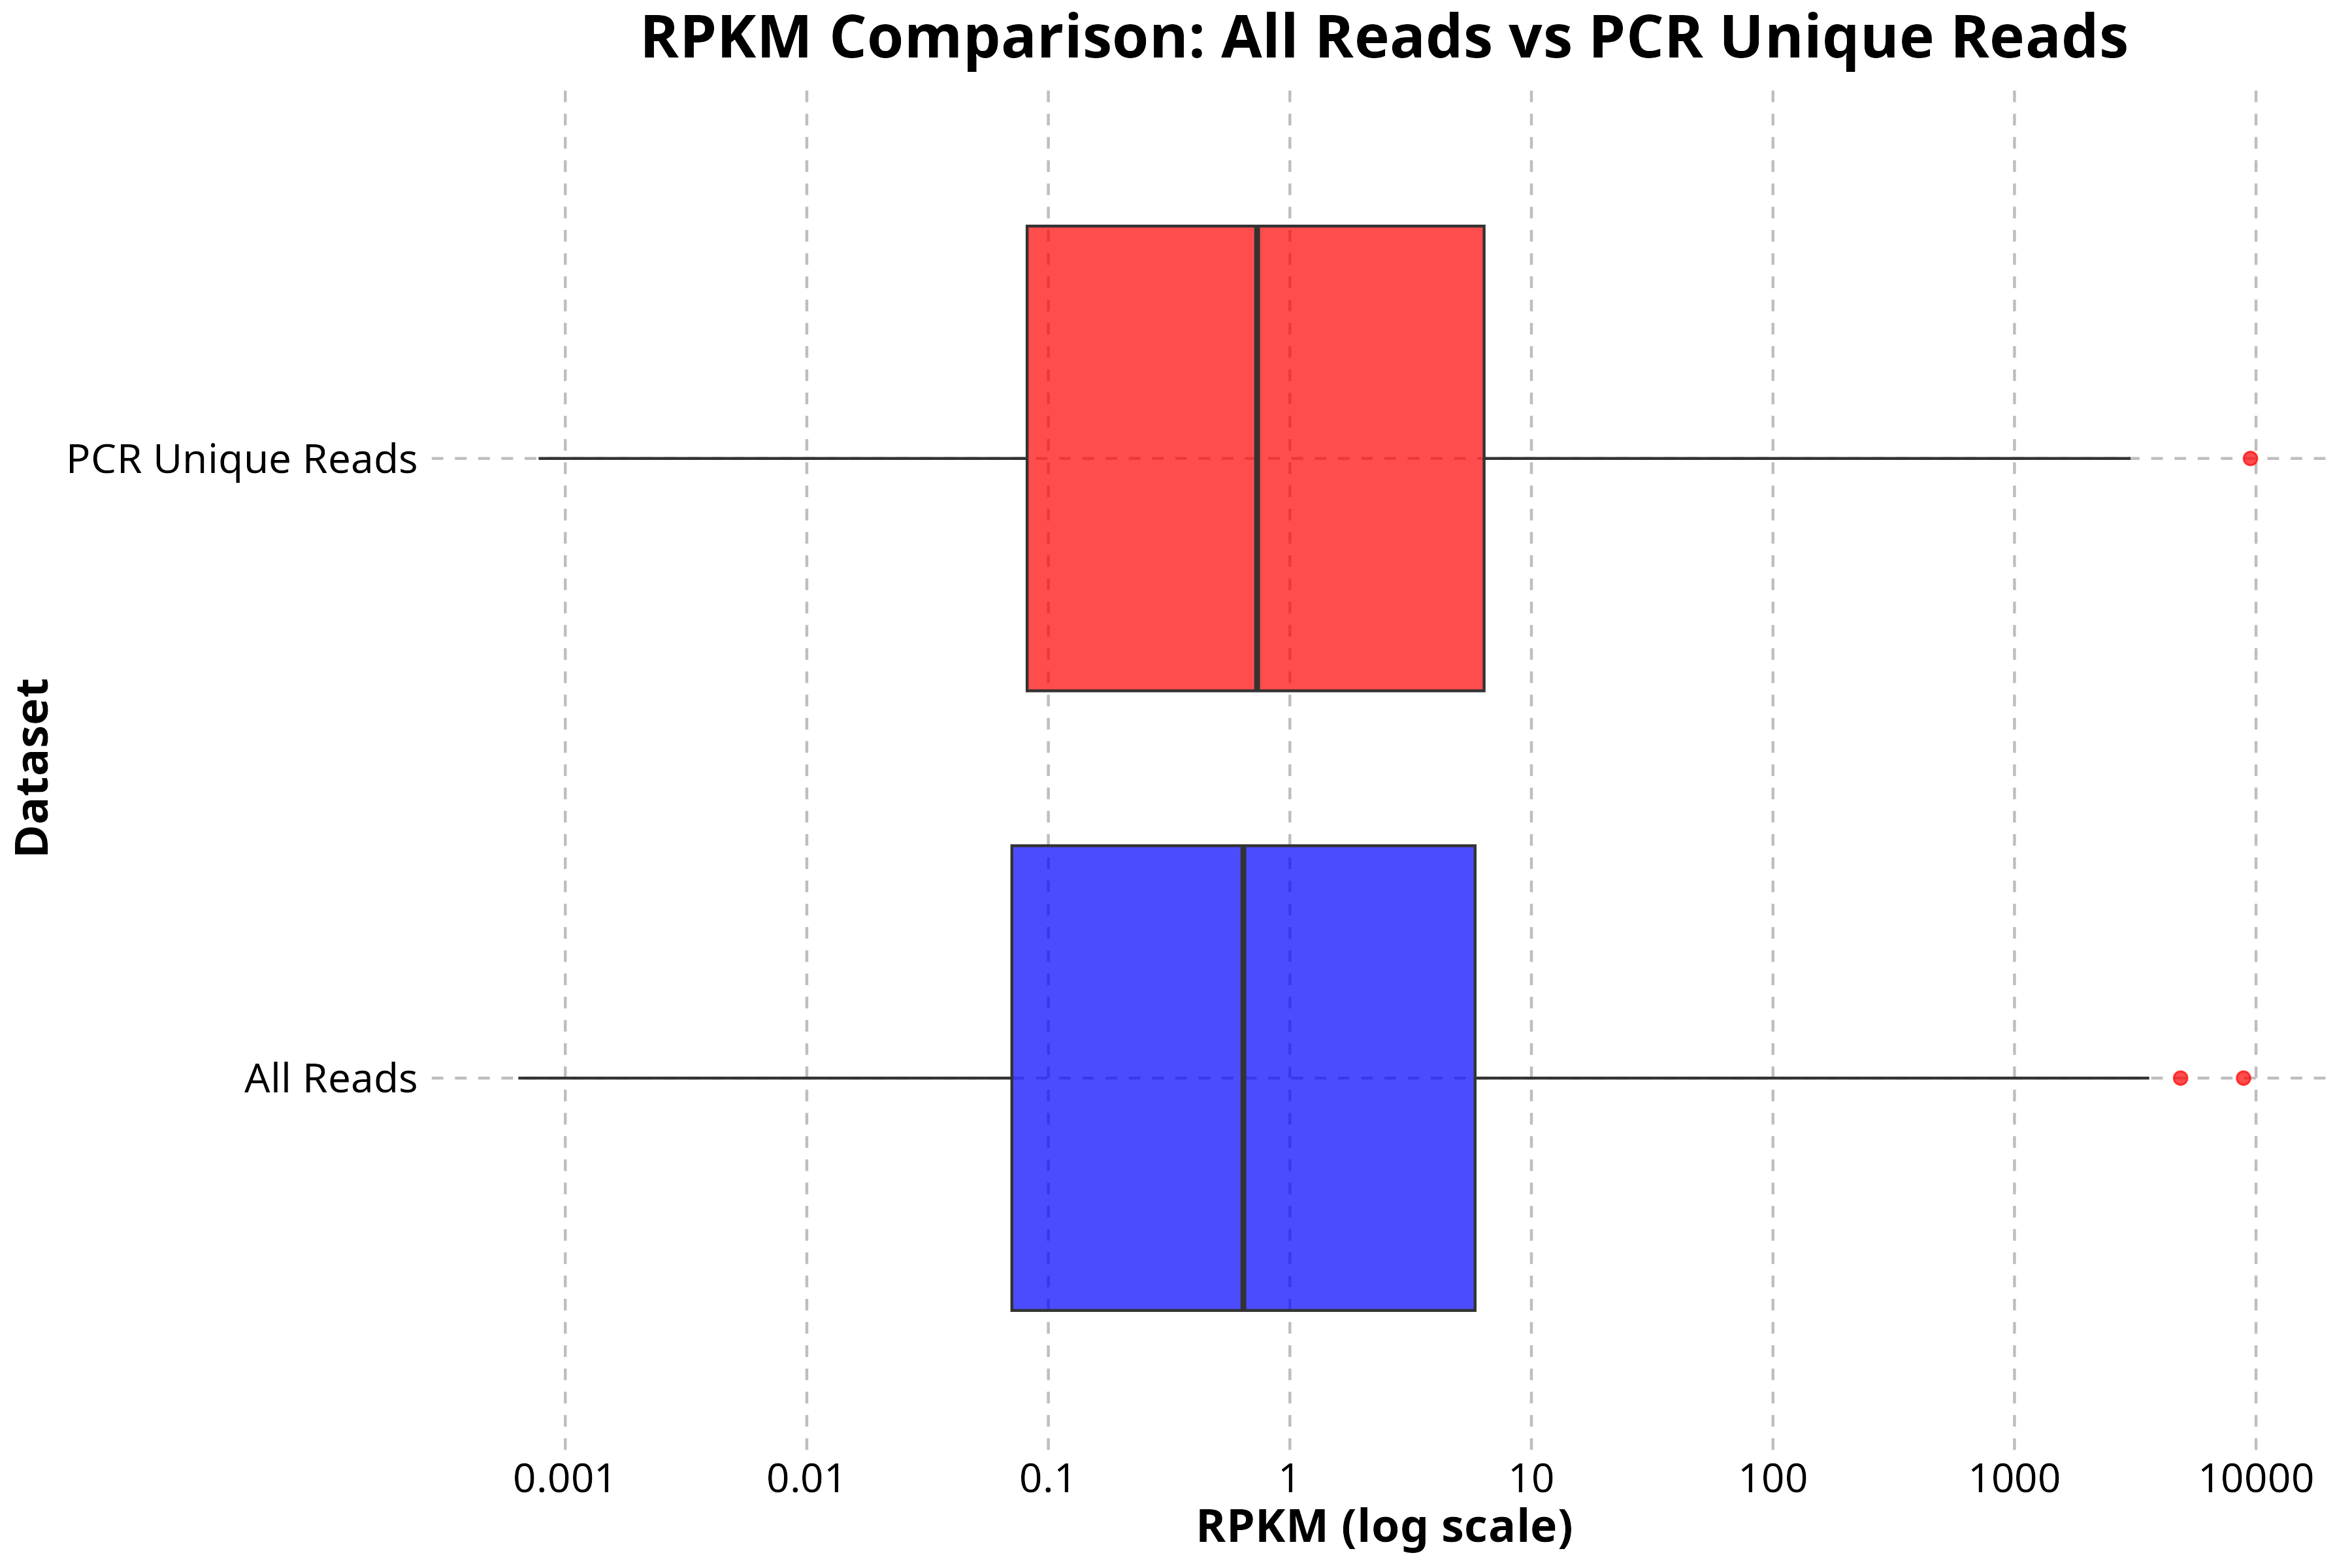
\includegraphics[width=0.85\textwidth]{./plots/ebna_hisat/Plots/rpkm_hist.png}
%     \caption{}
%     \label{fig:-plots-ebna_hisat-Plots-rpkm_hplot-png}
% \end{figure}
% \begin{figure}[htpb]
%     \centering
%     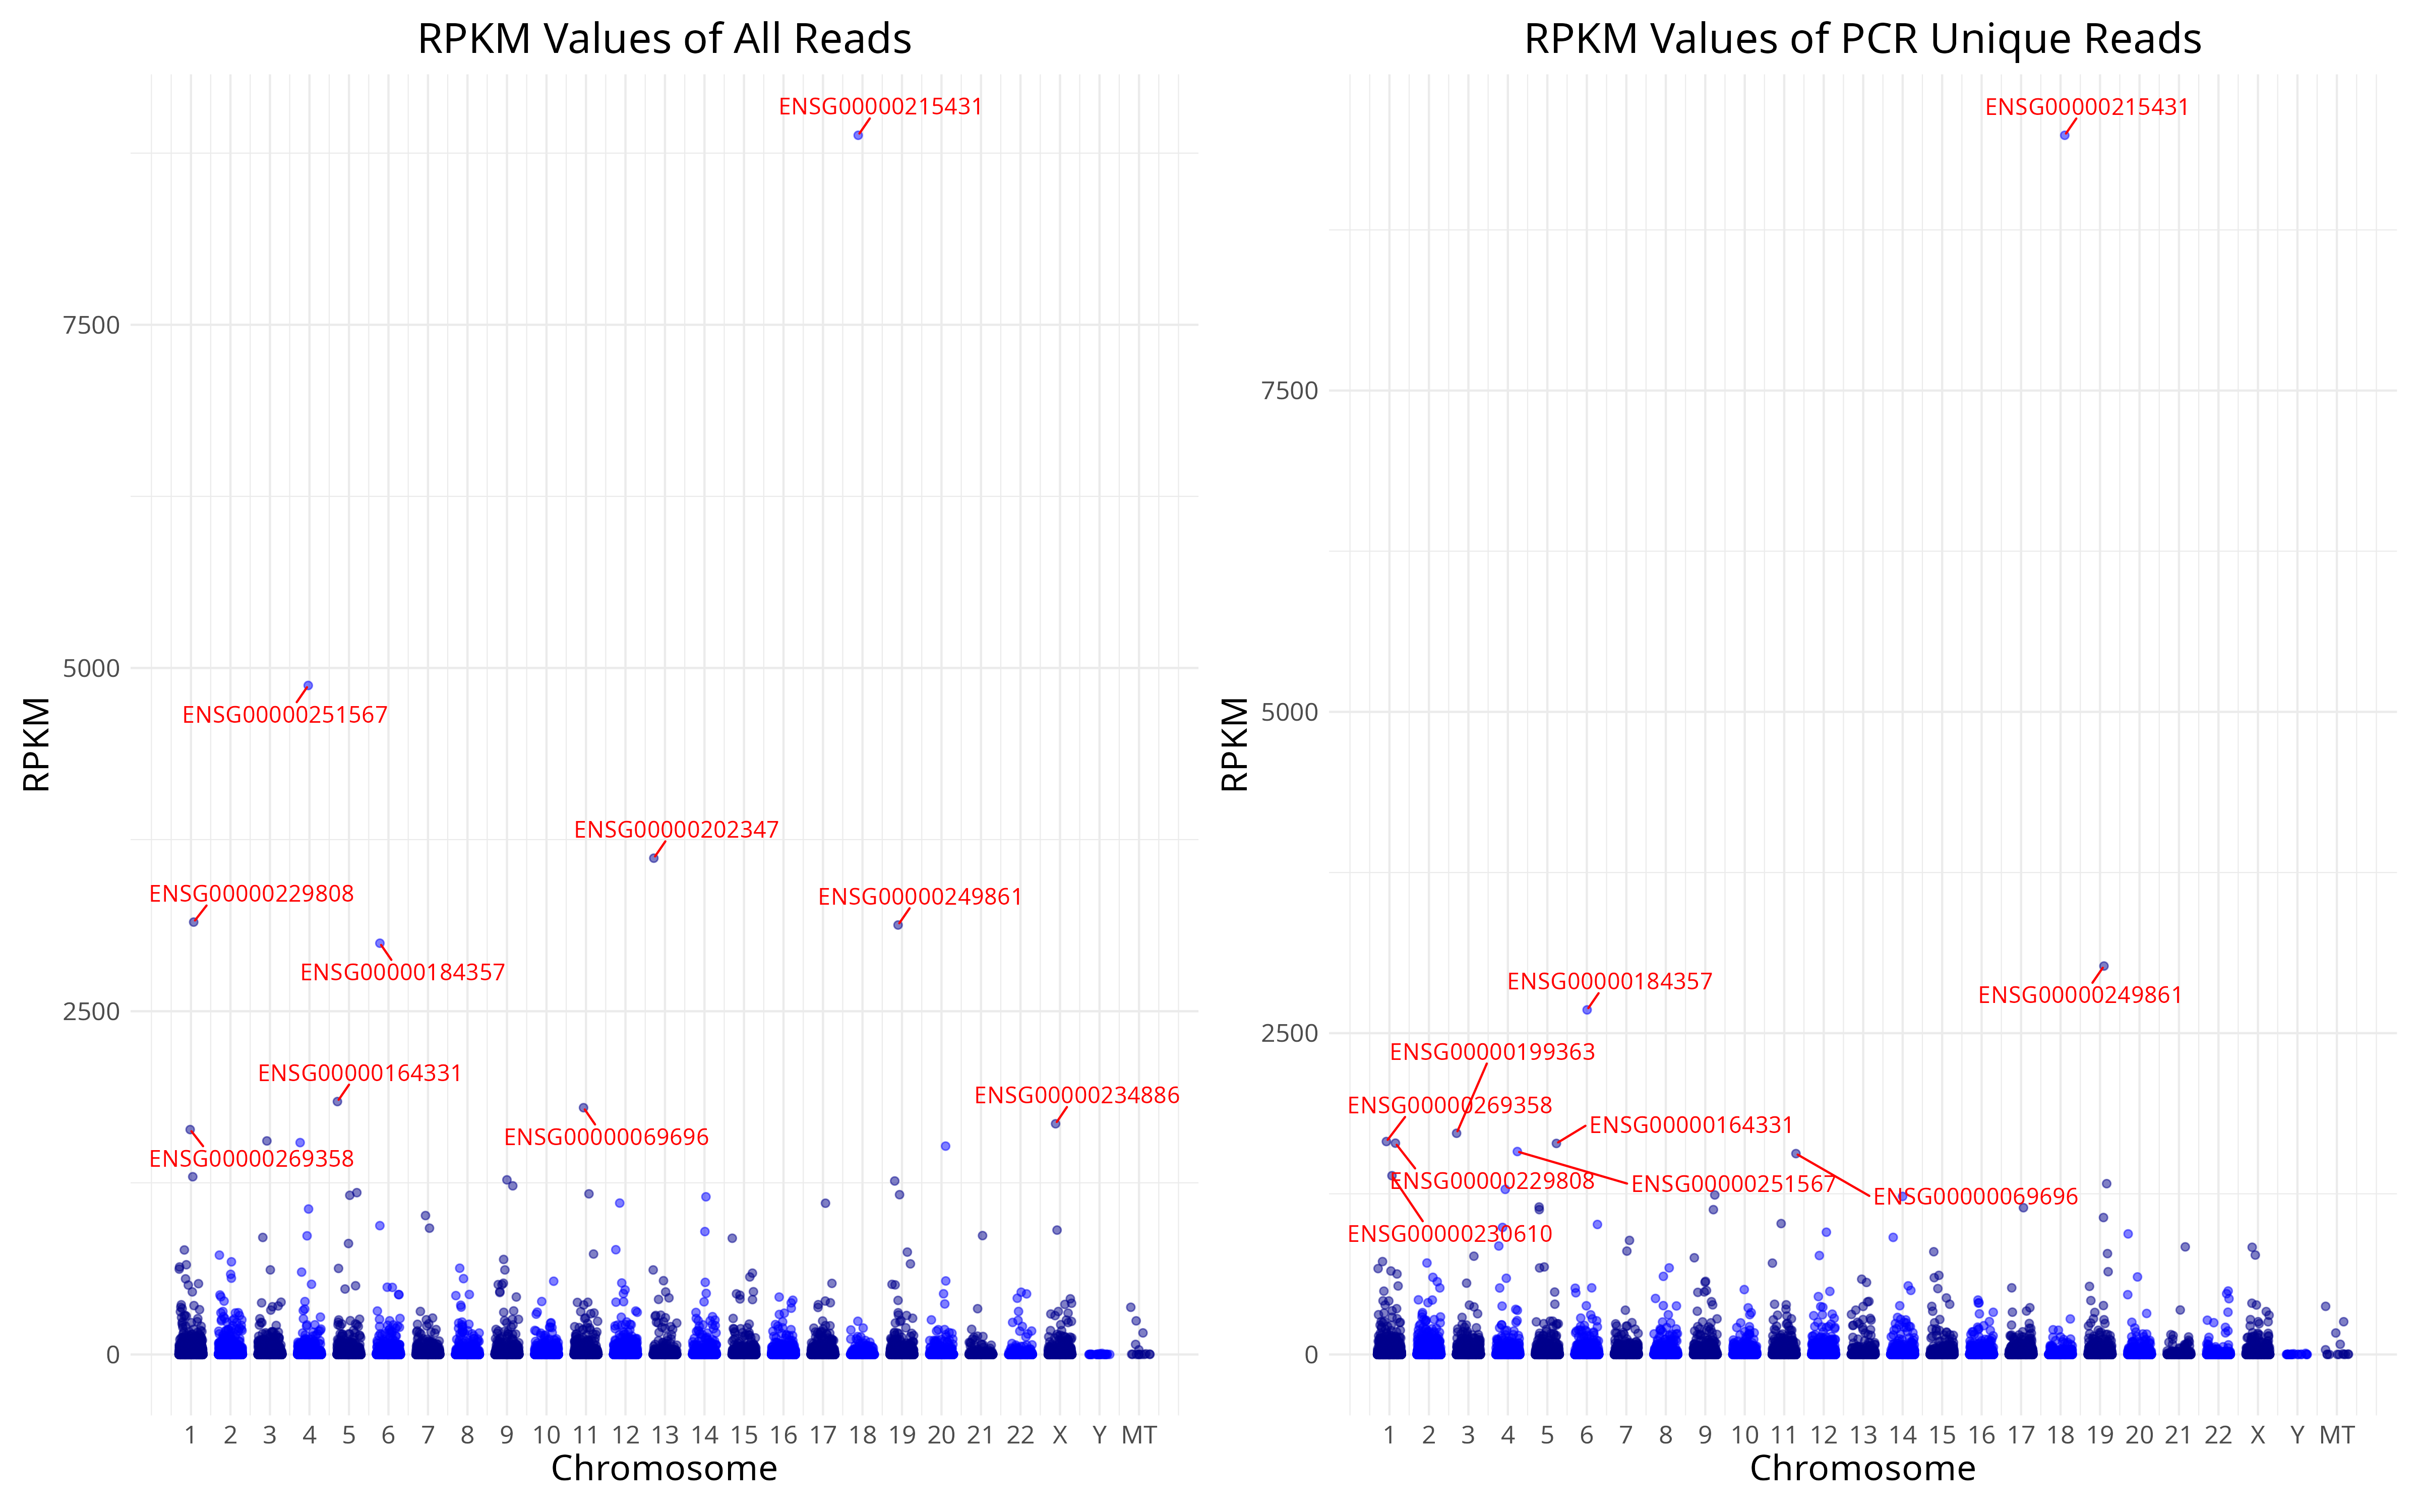
\includegraphics[width=0.85\textwidth]{./plots/ebna_hisat/Plots/rpkm_mplot.png}
%     \caption{}
%     \label{fig:-plots-ebna_hisat-Plots-rpkm_mplot-png}
% \end{figure}
% \begin{figure}[htpb]
%     \centering
%     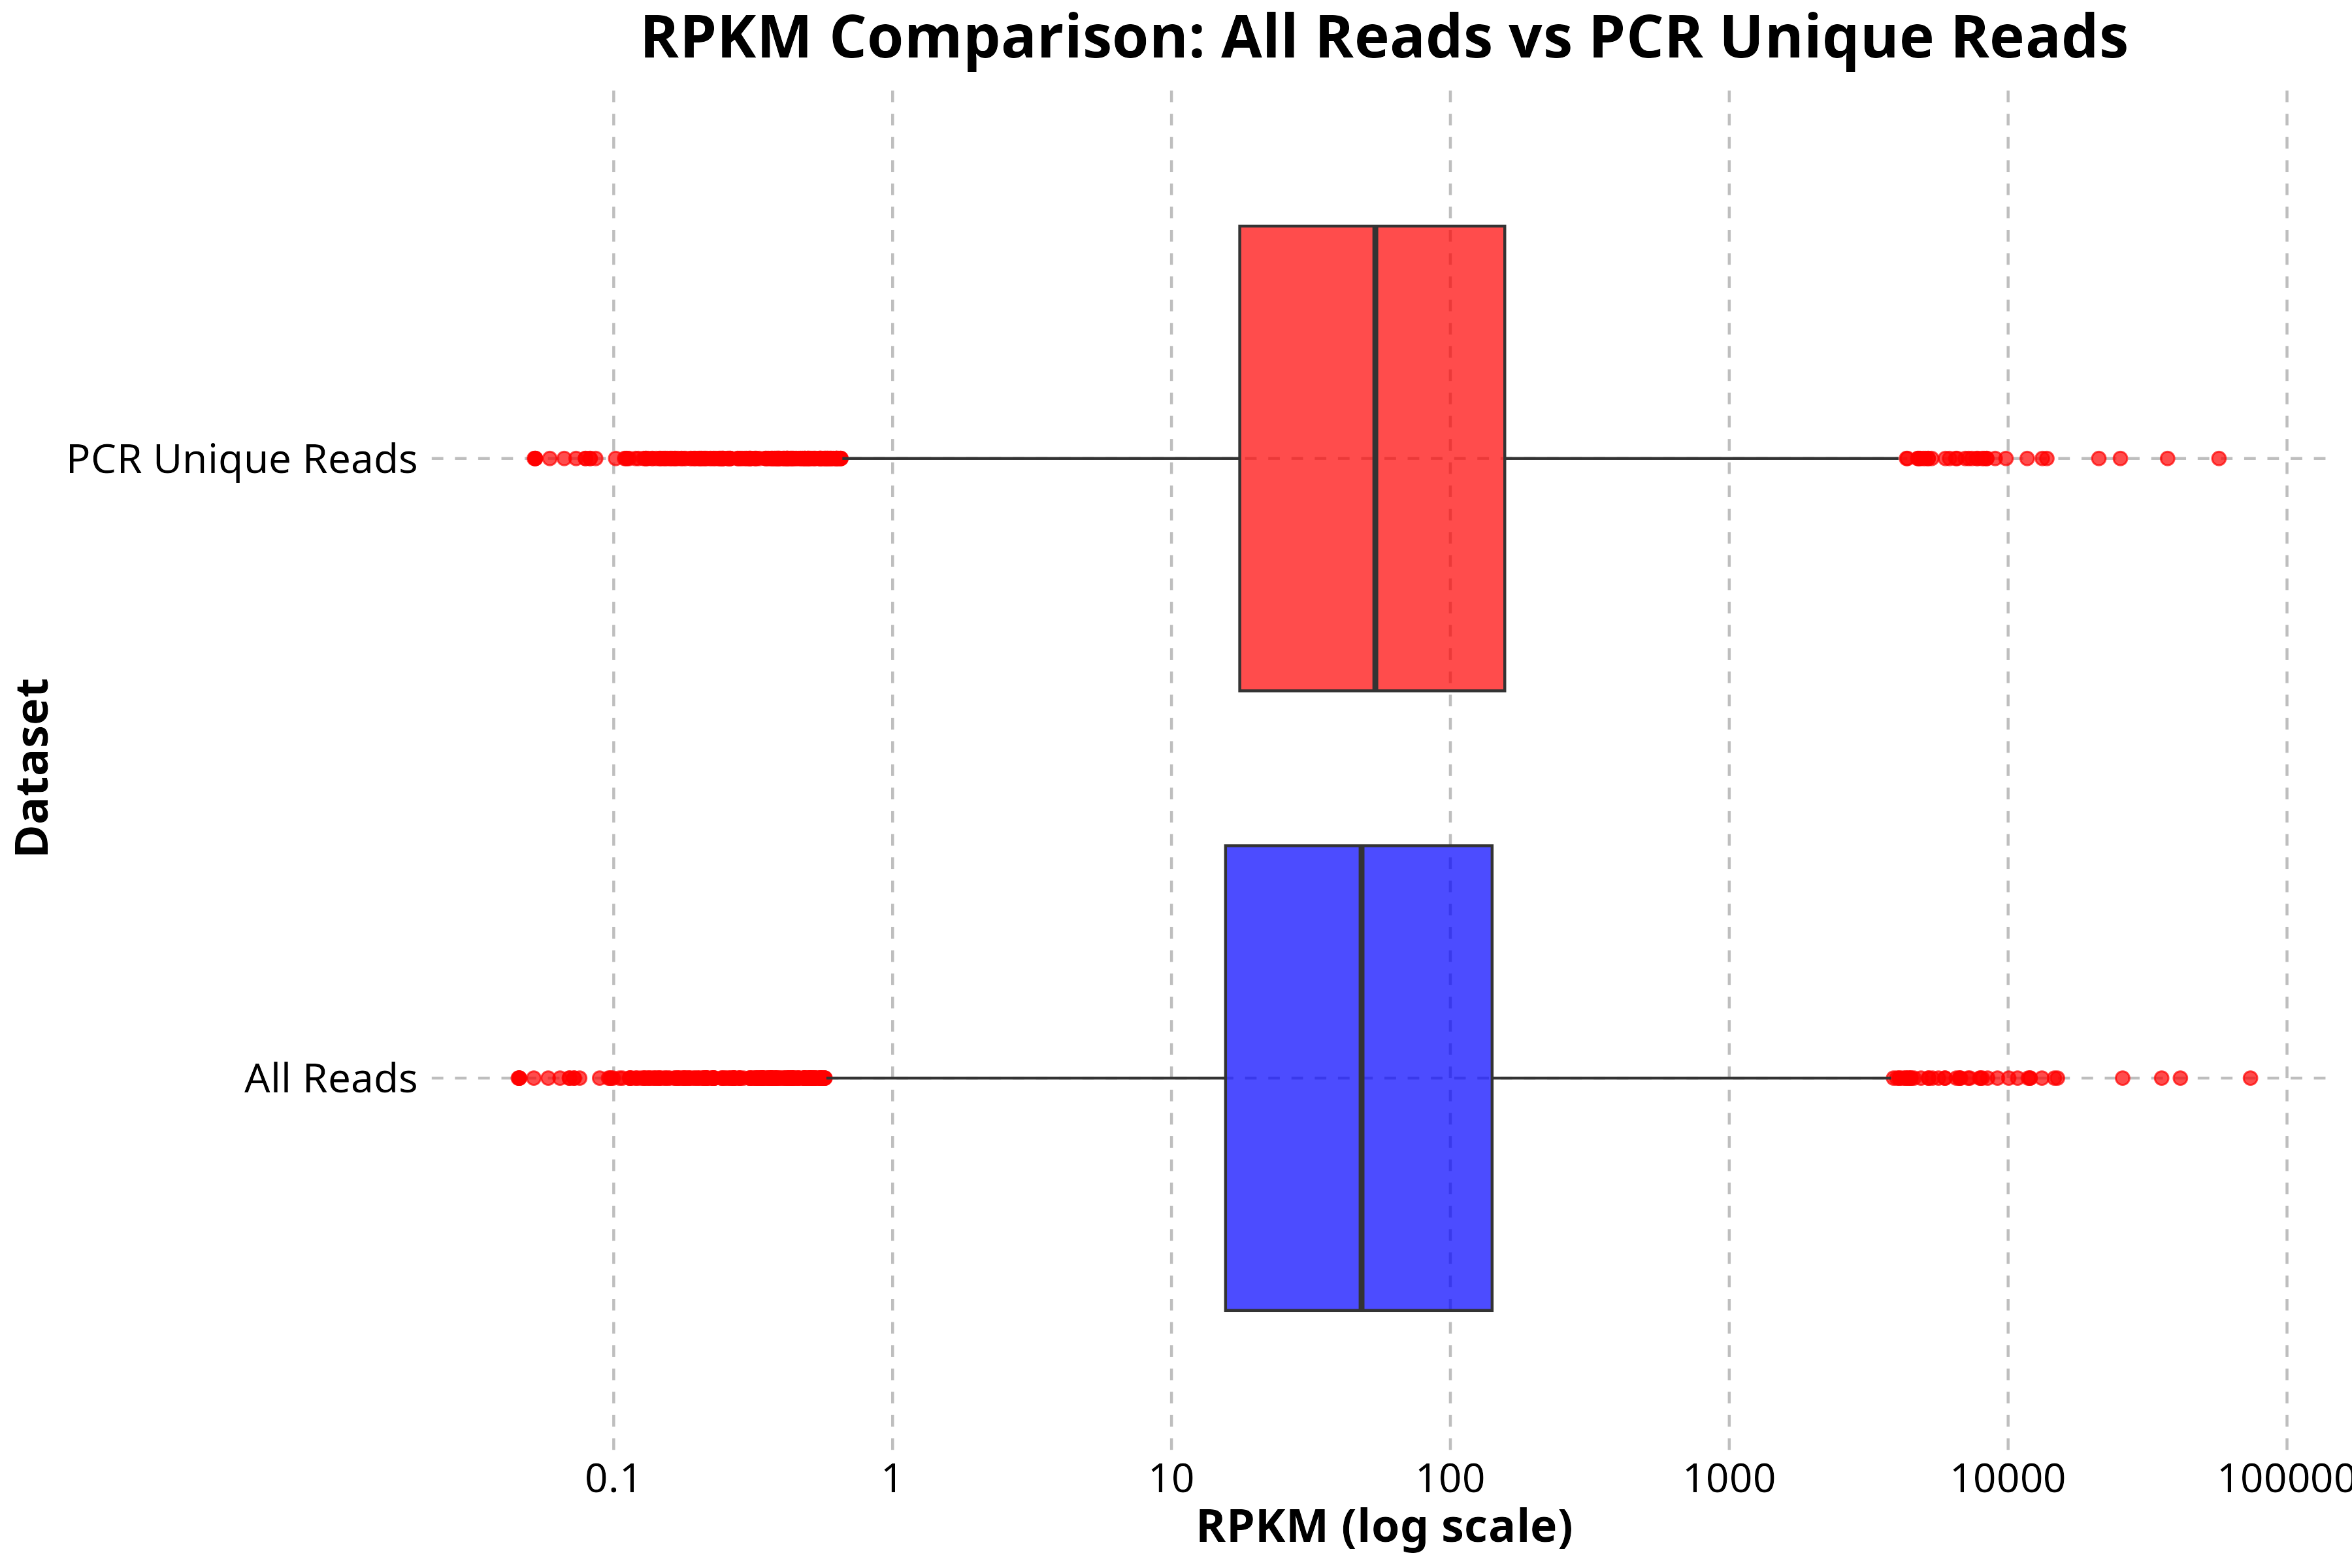
\includegraphics[width=0.85\textwidth]{./plots/nookaew_cm/Plots/rpkm_hist.png}
%     \caption{}
%     \label{fig:-plots-nookaew_cm-Plots-rpkm_hplot-png}
% \end{figure}
% \begin{figure}[htpb]
%     \centering
%     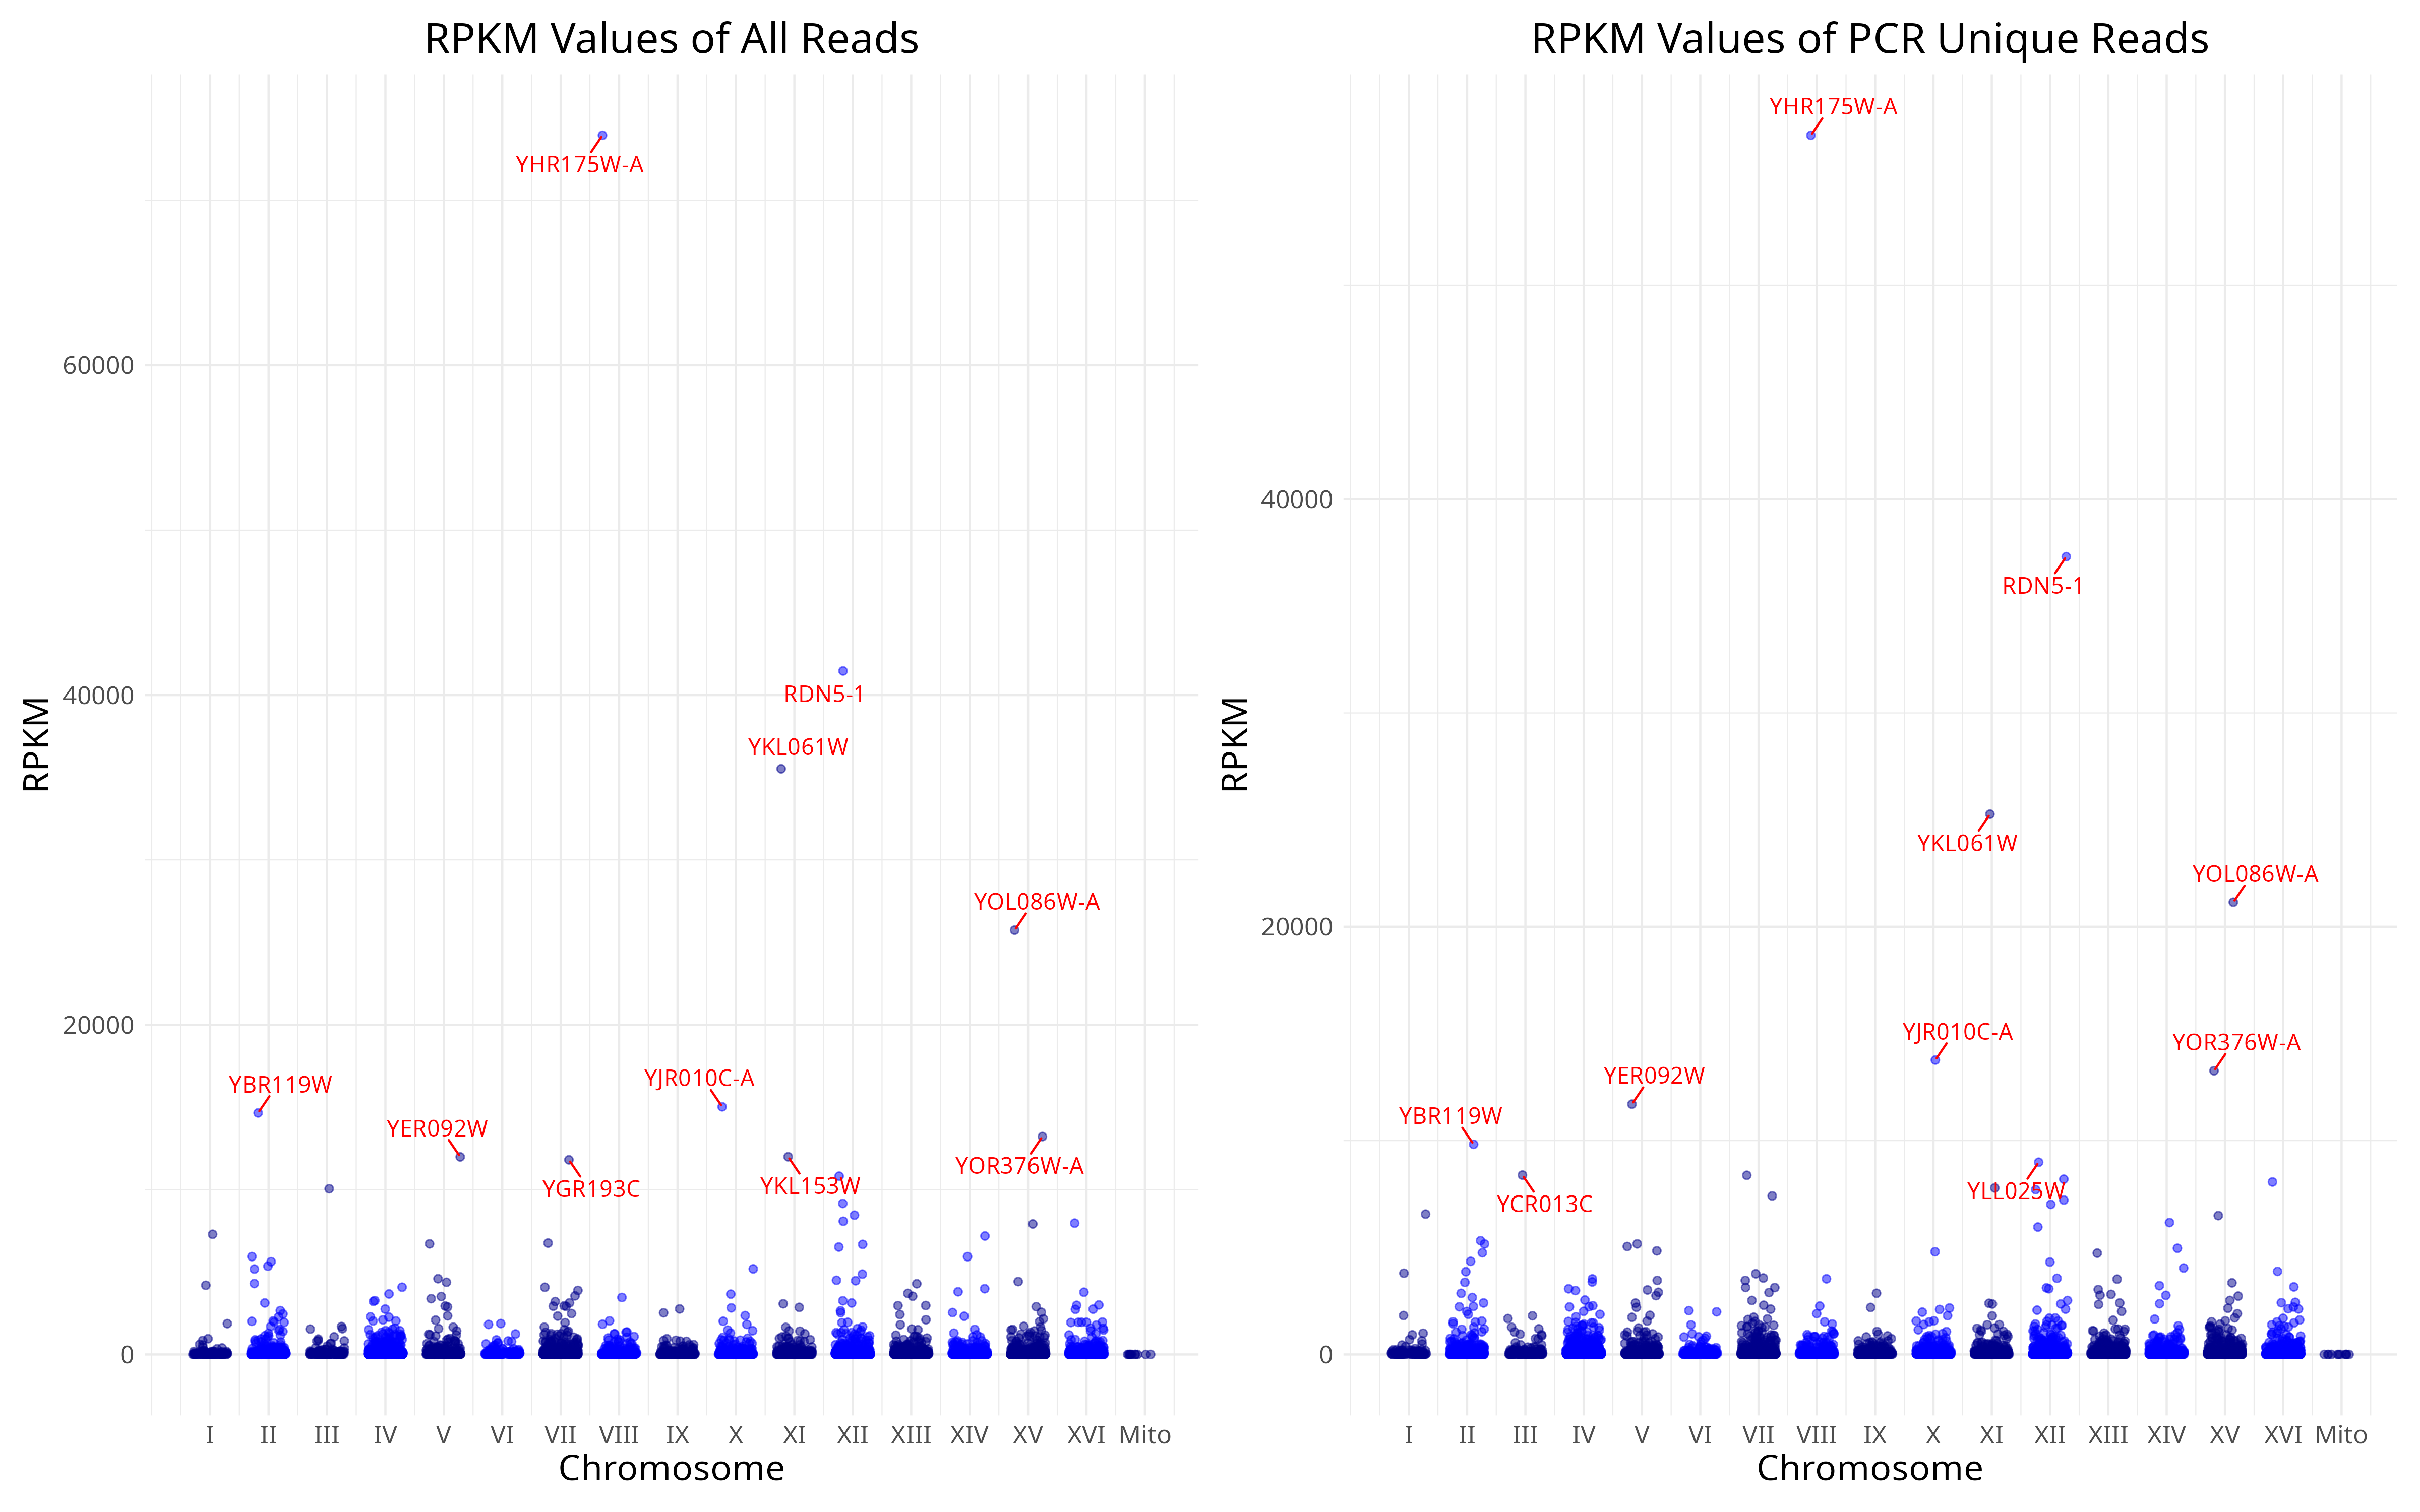
\includegraphics[width=0.85\textwidth]{./plots/nookaew_cm/Plots/rpkm_mplot.png}
%     \caption{}
%     \label{fig:-plots-nookaew_cm-Plots-rpkm_mplot-png}
% \end{figure}



% ------------------------------------------------------------------------------
\printbibliography
% ------------------------------------------------------------------------------


% ------------------------------------------------------------------------------
\newpage~\appendix
% ------------------------------------------------------------------------------

\section{Appendix Section}

hm 

Text goes here



\end{document}
